\begin{document}
    \subsection{Keyboard and Mouse Models}


    \subsection{Faceial Models}

    Our deep learning models managed to achieve much better results compared to the classical models. 
    This improvement makes sense when we consider the data they use. Facial data carries features that are more 
    indicative of a user's emotional state compared to mouse and keyboard features, such as average press duration or mouse angle.

    \begin{figure}[htp]
        \centering
        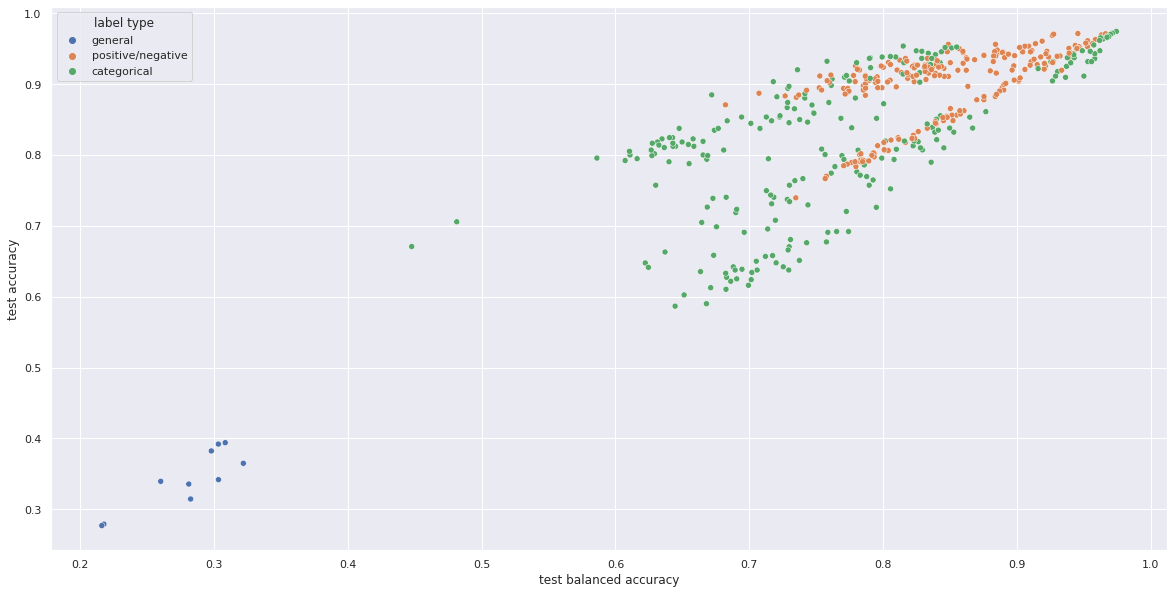
\includegraphics[width=14cm]{figures/results/nn_acc}   
        \caption{We can see the balanced and unbalanced accuracies of all the "Emotion Net Nano" based models we trained in this plot.
        We can also see the colors separating the models into three categories, models predicting positive/negative labels, models predicting
        categorical labels, and the general models that were trained on all the participants at once.}
        \label{fig:nn_acc} 
    \end{figure}

    When we look at the categorical and positive/negative Label types \ref{fig:nn_acc}, we can clearly see an improvement over 
    the classical models, where even the worst of the personal models achieve better performance than the best classical models.
    On the other hand, we can also see that the general models, those trained on all the participants' data, achieve inferior results, 
    even compared to the classical models. On the other hand, we can also see that the general models, 
    those trained on all the participants' data, achieve inferior results, even compared to the classical models when trying 
    to generalize over different people. The inability to generalize facial features is likely due to the minimal data 
    set and our model being very small and simple in terms of trainable parameters. This is not necessarily a bad thing. 
    We intended to create tiny and efficient models that would train on a user's computer and make predictions very easily and quickly.

    \begin{figure}[htp]
        \centering
        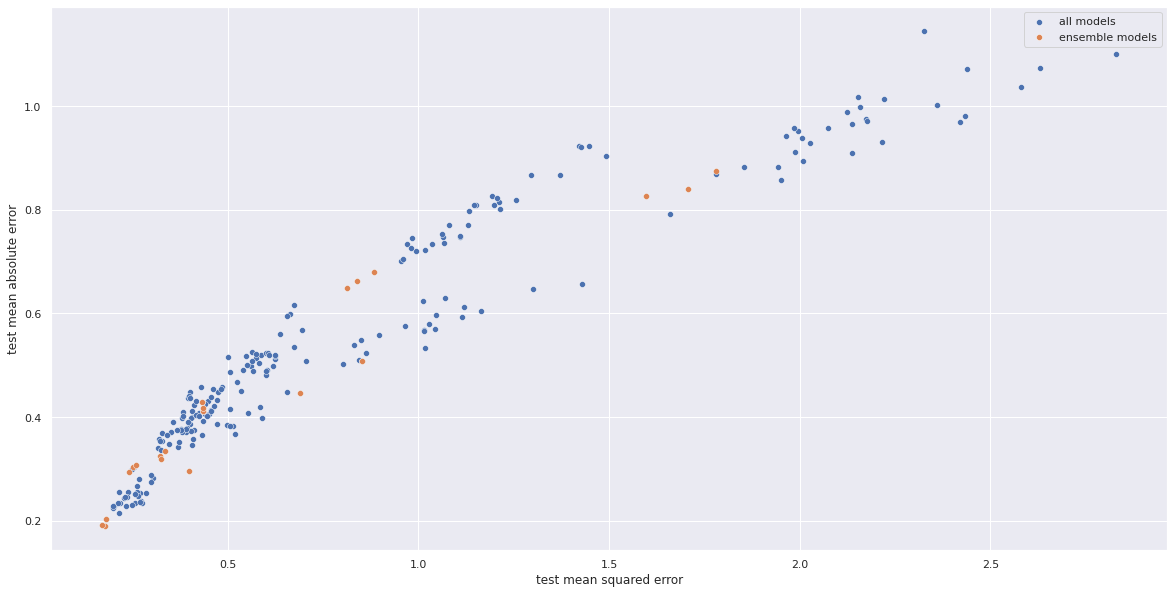
\includegraphics[width=14cm]{figures/results/nn_err}   
        \caption{Here we can see the mean absolute and squared errors of allt he regression models, where the ensemble models are highlated in orange}
        \label{fig:nn_err} 
    \end{figure}


    The story is a bit different when looking at the VAD models \ref{fig:nn_err}. First, we can notice that the variance is very high. 
    Secondly, we have excellent models that achieve a Mean absolute error of less than 0.2, which is much better than the classical models. However, 
    we also have quite a few models that achieve results not much better, even as bad as an MAE of one. Though if we only look at the ensemble models, 
    we can see that they are a little more consistent. We constructed confidence intervals for all the models and just the ensemble models, 
    and with a confidence of 0.95, we can say that all the models are in the range $(0.08, 1)$ and $(0.03, 0.86)$ for ensemble models. Both intervals 
    have incredibly impressive lower bounds, but the upper bound is a little high. 

    \subsection{Ensemble}
\end{document}